\subsubsubsection*{6.2.8 Thiết kế và xây dựng SmartWater Admin}

Trong cùng tuần triển khai Device Monitor, sinh viên hoàn thiện giao diện quản trị SmartWater Admin nhằm khai thác dữ liệu nghiệp vụ và telemetry đã được chuẩn hóa. Ứng dụng được xây dựng bằng Laravel, bảo vệ các route quản trị bằng middleware xác thực và tổ chức theo chuỗi xử lý \textit{Route $\rightarrow$ Controller $\rightarrow$ Service $\rightarrow$ Eloquent Model $\rightarrow$ Blade View}.

Các công việc chính gồm:

\begin{itemize}
    \item Hoàn thiện trang đăng nhập và dashboard tổng quan.
    \item Xây dựng các màn hình quản lý sản phẩm, kho và lô hàng.
    \item Xây dựng các màn hình khách hàng, hợp đồng và hồ sơ khách hàng.
    \item Xây dựng các màn hình quản lý thiết bị, MCU và telemetry.
    \item Xây dựng các màn hình nhân viên, lịch sử hoạt động và hồ sơ người dùng.
    \item Đối chiếu giao diện với route, controller, service và dữ liệu MySQL hiện có.
\end{itemize}

\subsubsubsection*{6.2.8.1 Kiến trúc dashboard}

SmartWater Admin là ứng dụng Laravel nguyên khối phục vụ quản trị. Sau khi người dùng đăng nhập, route \path|/| hoặc \path|/dashboard| gọi \texttt{DashboardController::index}. Controller sử dụng \texttt{DashboardService} để lấy các chỉ số KPI, phân bố trạng thái thiết bị, dữ liệu khách hàng theo tháng, bảo trì theo tháng, hoạt động gần đây và hợp đồng sắp hết hạn; sau đó truyền dữ liệu tới Blade view dashboard.

Dashboard tổng hợp số khách hàng, sản phẩm, thiết bị, thiết bị đang hoạt động, thiết bị bảo trì và hợp đồng còn hiệu lực từ database. Các biểu đồ sử dụng dữ liệu truy vấn theo tháng hoặc theo trạng thái thiết bị. Phần xu hướng phần trăm trên KPI hiện là giá trị trình bày cố định, vì vậy chỉ được dùng để minh họa giao diện và cần được thay bằng phép so sánh dữ liệu lịch sử khi triển khai hoàn chỉnh.

\subsubsubsection*{6.2.8.2 Giao diện xác thực và dashboard tổng quan}

Trang đăng nhập là điểm vào của hệ thống. Sau khi xác thực thành công, người dùng được chuyển đến dashboard để quan sát chỉ số tổng quan và truy cập các module quản trị từ sidebar.

\begin{figure}[H]
    \centering
    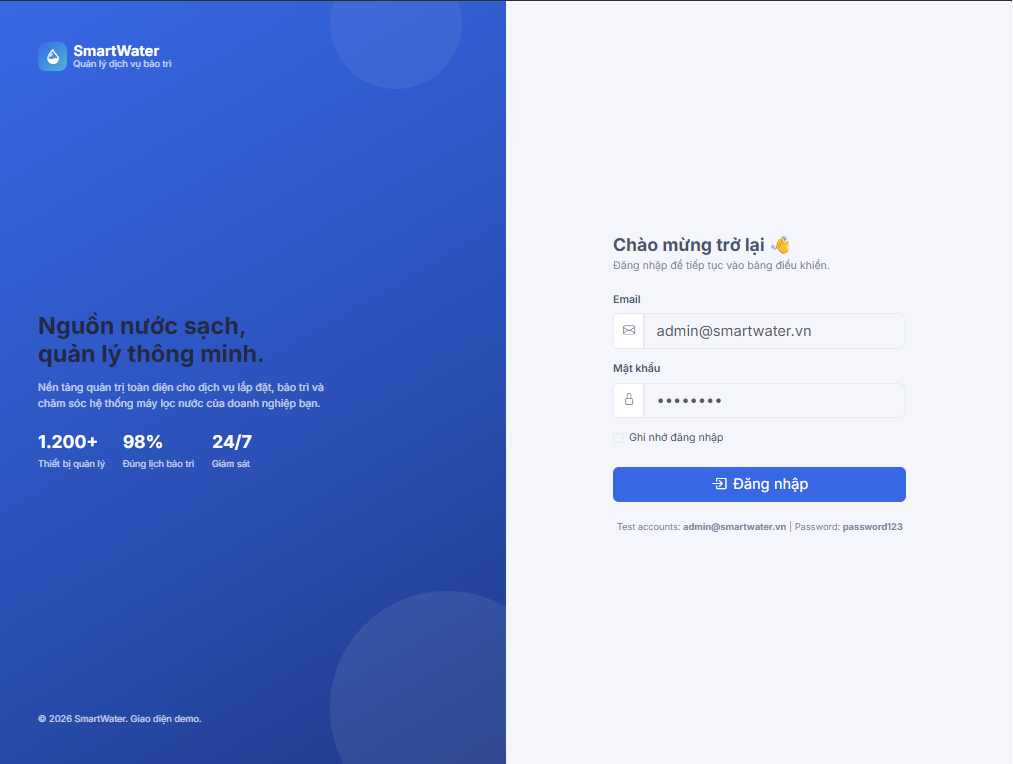
\includegraphics[width=0.90\linewidth]{include/web-UI/smartwater-admin-login.png}
    \caption{Giao diện đăng nhập SmartWater Admin}
    \label{fig:week7-admin-login}
\end{figure}

\begin{figure}[H]
    \centering
    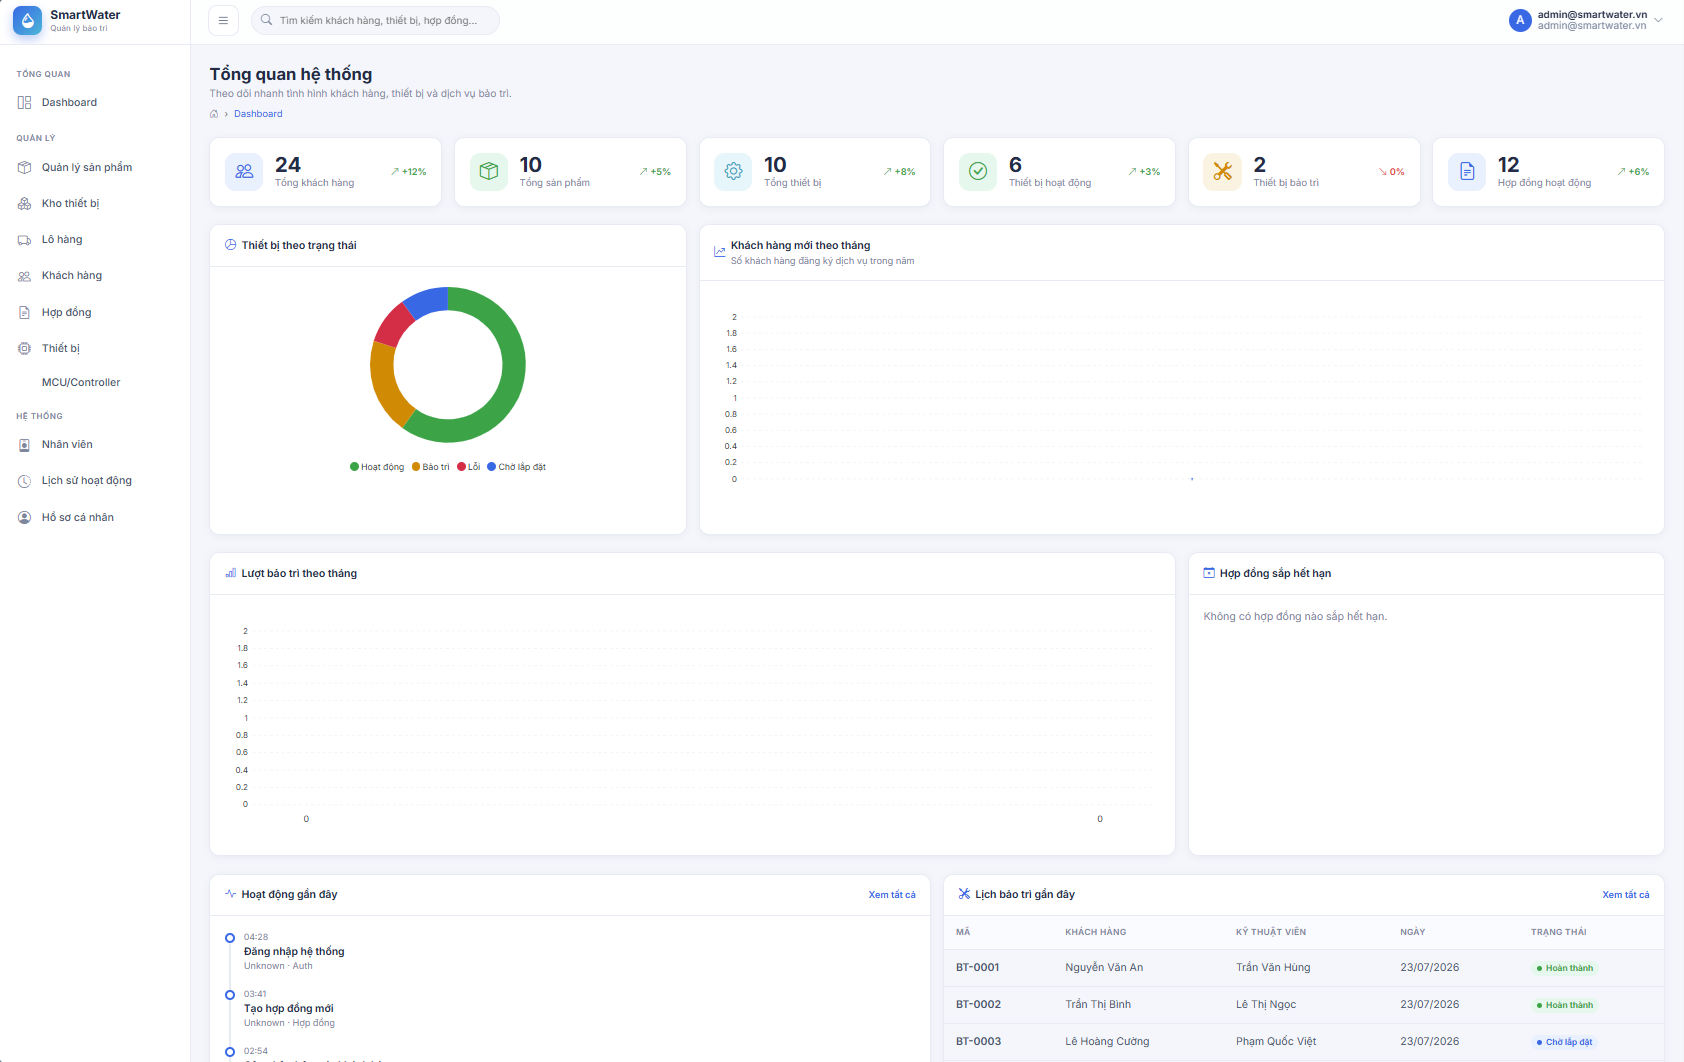
\includegraphics[width=0.95\linewidth]{include/web-UI/smartwater-admin-main.png}
    \caption{Dashboard tổng quan SmartWater Admin}
    \label{fig:week7-admin-dashboard}
\end{figure}

\subsubsubsection*{6.2.8.3 Quản lý danh mục, sản phẩm, kho và lô hàng}

Module sản phẩm là dữ liệu nền cho thiết bị và kho. Mỗi sản phẩm thuộc một danh mục; tồn kho được quản lý theo sản phẩm, còn lô hàng và chi tiết lô hàng hỗ trợ truy vết nguồn nhập. Các màn hình danh sách cung cấp khả năng xem, tìm kiếm và thao tác quản trị theo route của từng module.

\begin{figure}[H]
    \centering
    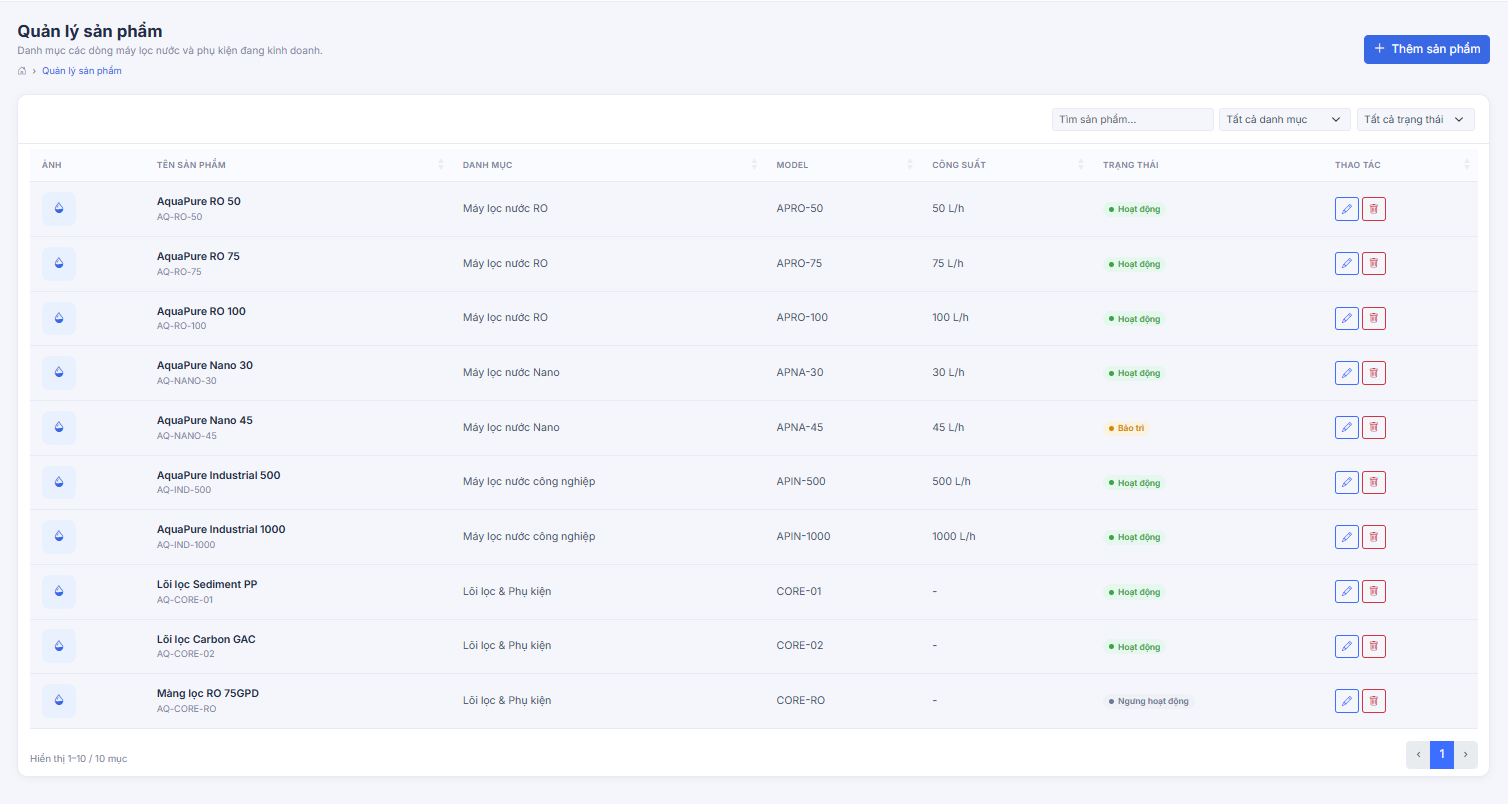
\includegraphics[width=0.90\linewidth]{include/web-UI/smartwater-admin-product.png}
    \caption{Giao diện quản lý sản phẩm}
    \label{fig:week7-admin-product}
\end{figure}

\begin{figure}[H]
    \centering
    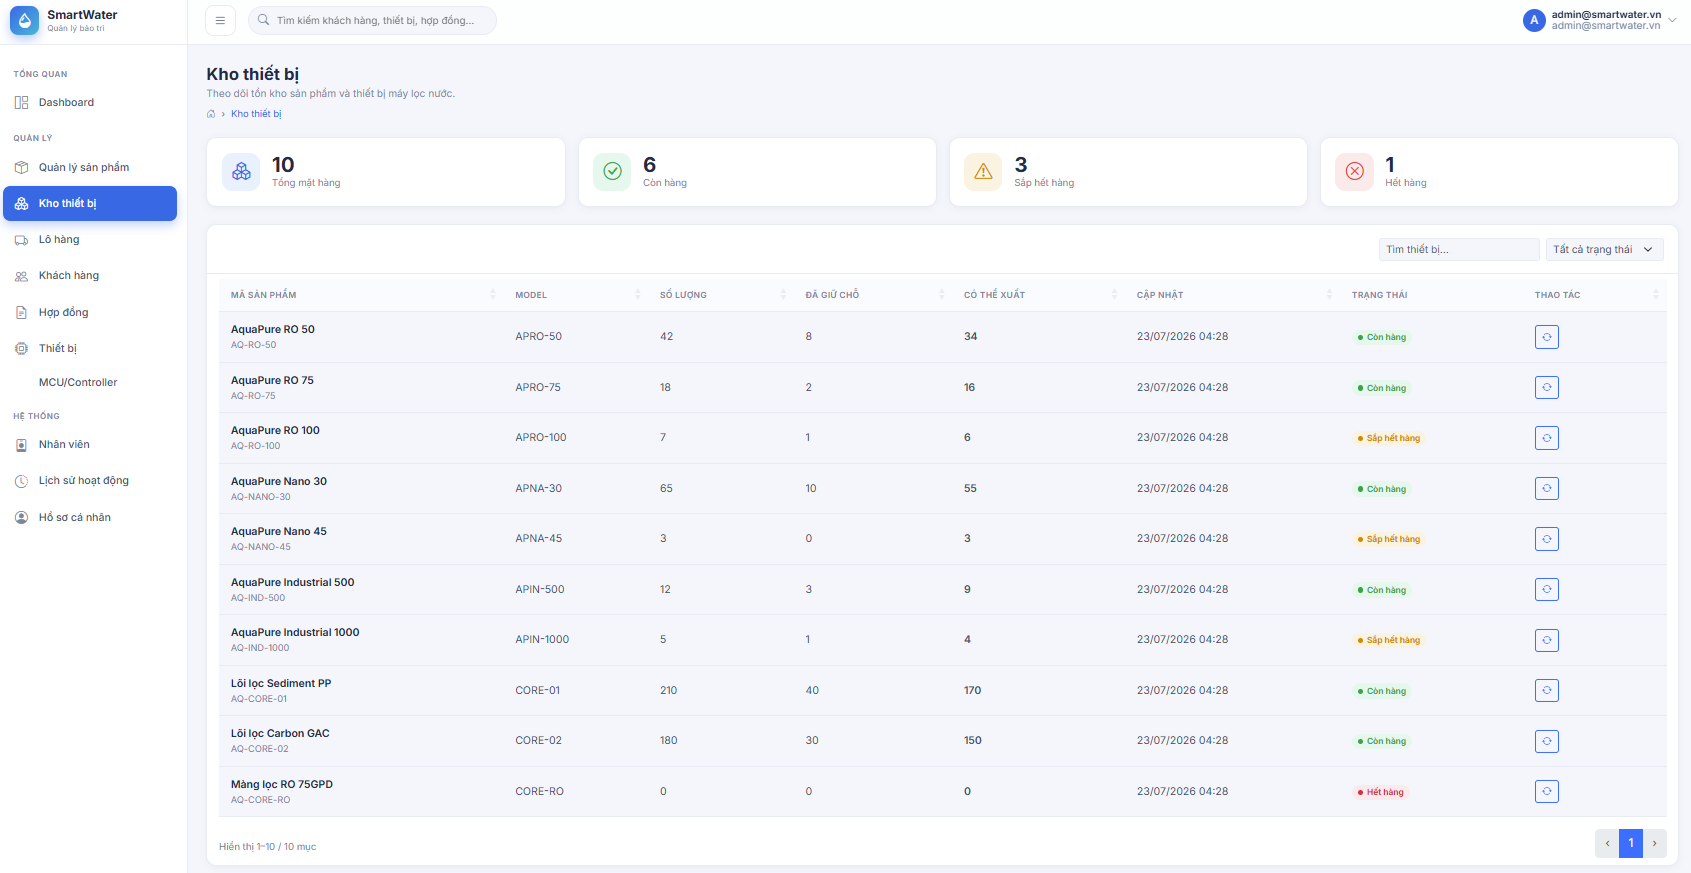
\includegraphics[width=0.90\linewidth]{include/web-UI/smartwater-admin-inventory.png}
    \caption{Giao diện quản lý tồn kho}
    \label{fig:week7-admin-inventory}
\end{figure}

\begin{figure}[H]
    \centering
    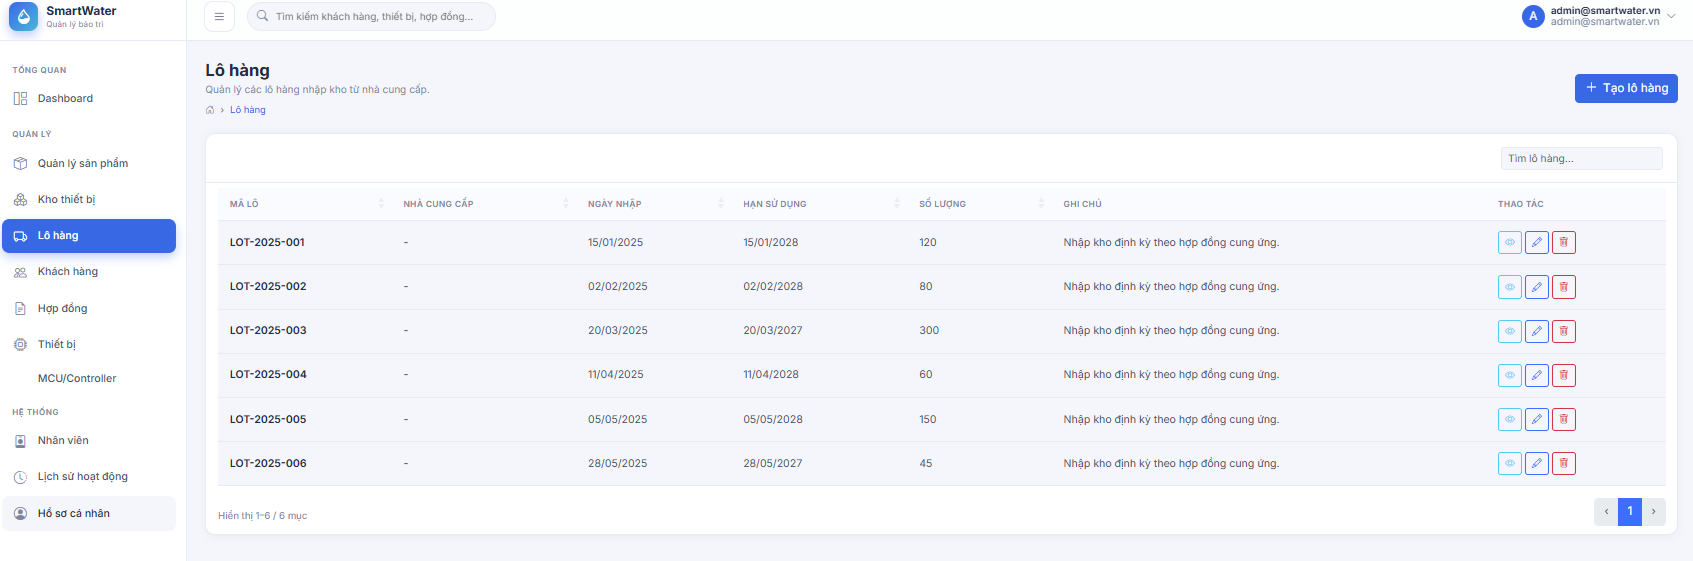
\includegraphics[width=0.90\linewidth]{include/web-UI/smartwater-admin-batch.png}
    \caption{Giao diện quản lý lô hàng}
    \label{fig:week7-admin-batch}
\end{figure}

\subsubsubsection*{6.2.8.4 Quản lý khách hàng và hợp đồng}

Nhóm chức năng khách hàng và hợp đồng thể hiện dữ liệu nghiệp vụ xuyên suốt quá trình lắp đặt và vận hành máy lọc nước. Một khách hàng có thể có nhiều hợp đồng; thiết bị được gắn với khách hàng và hợp đồng phù hợp để hỗ trợ truy vết khi xem thông tin vận hành hoặc lịch sử bảo trì.

\begin{figure}[H]
    \centering
    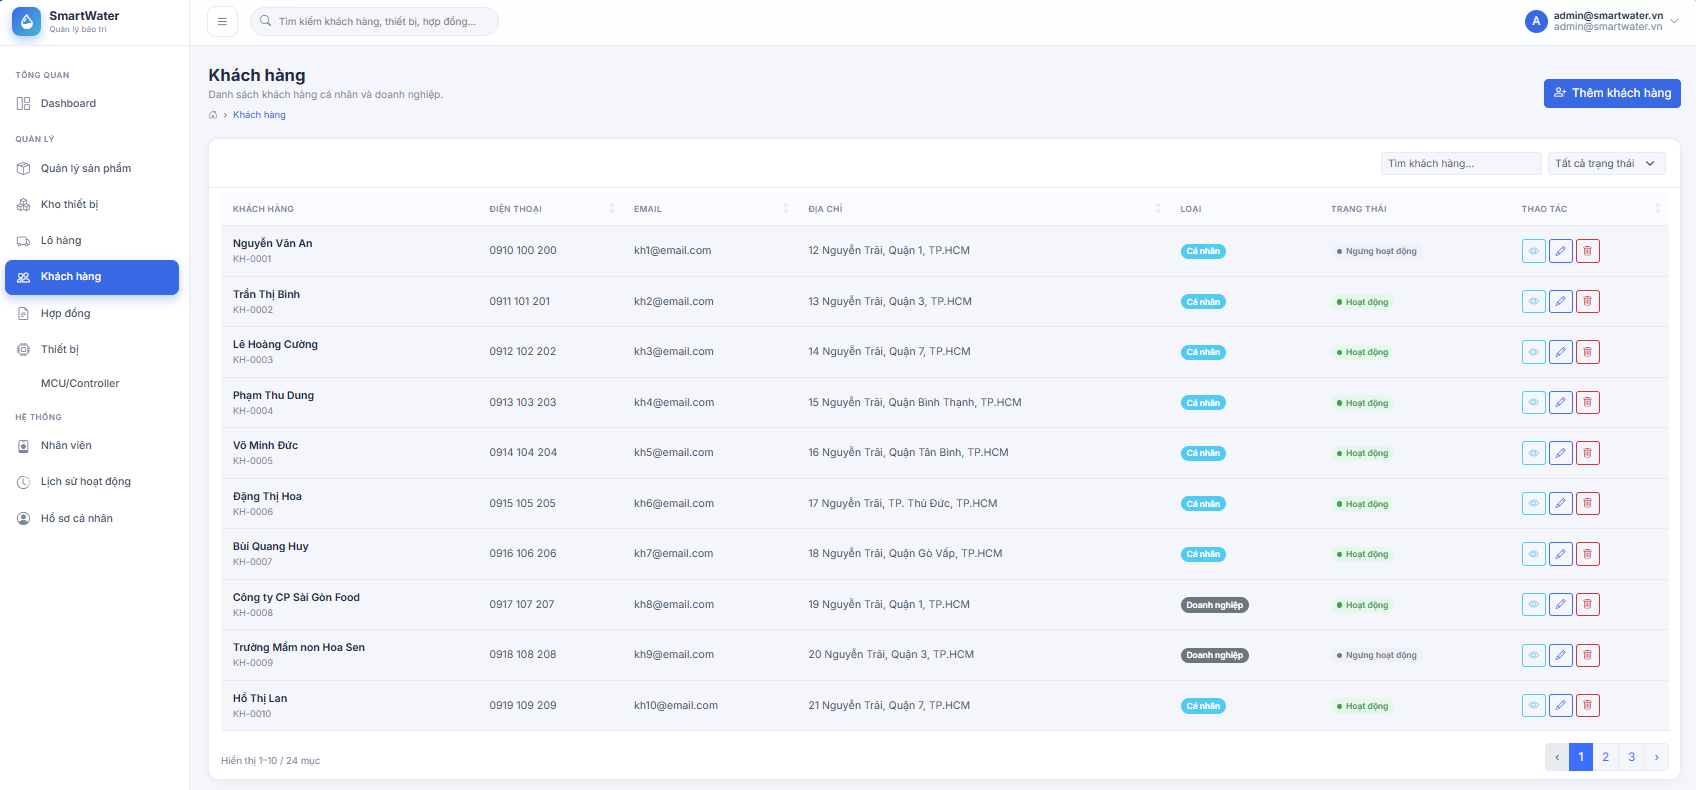
\includegraphics[width=0.90\linewidth]{include/web-UI/smartwater-admin-customer.png}
    \caption{Danh sách khách hàng trong SmartWater Admin}
    \label{fig:week7-admin-customer}
\end{figure}

\begin{figure}[H]
    \centering
    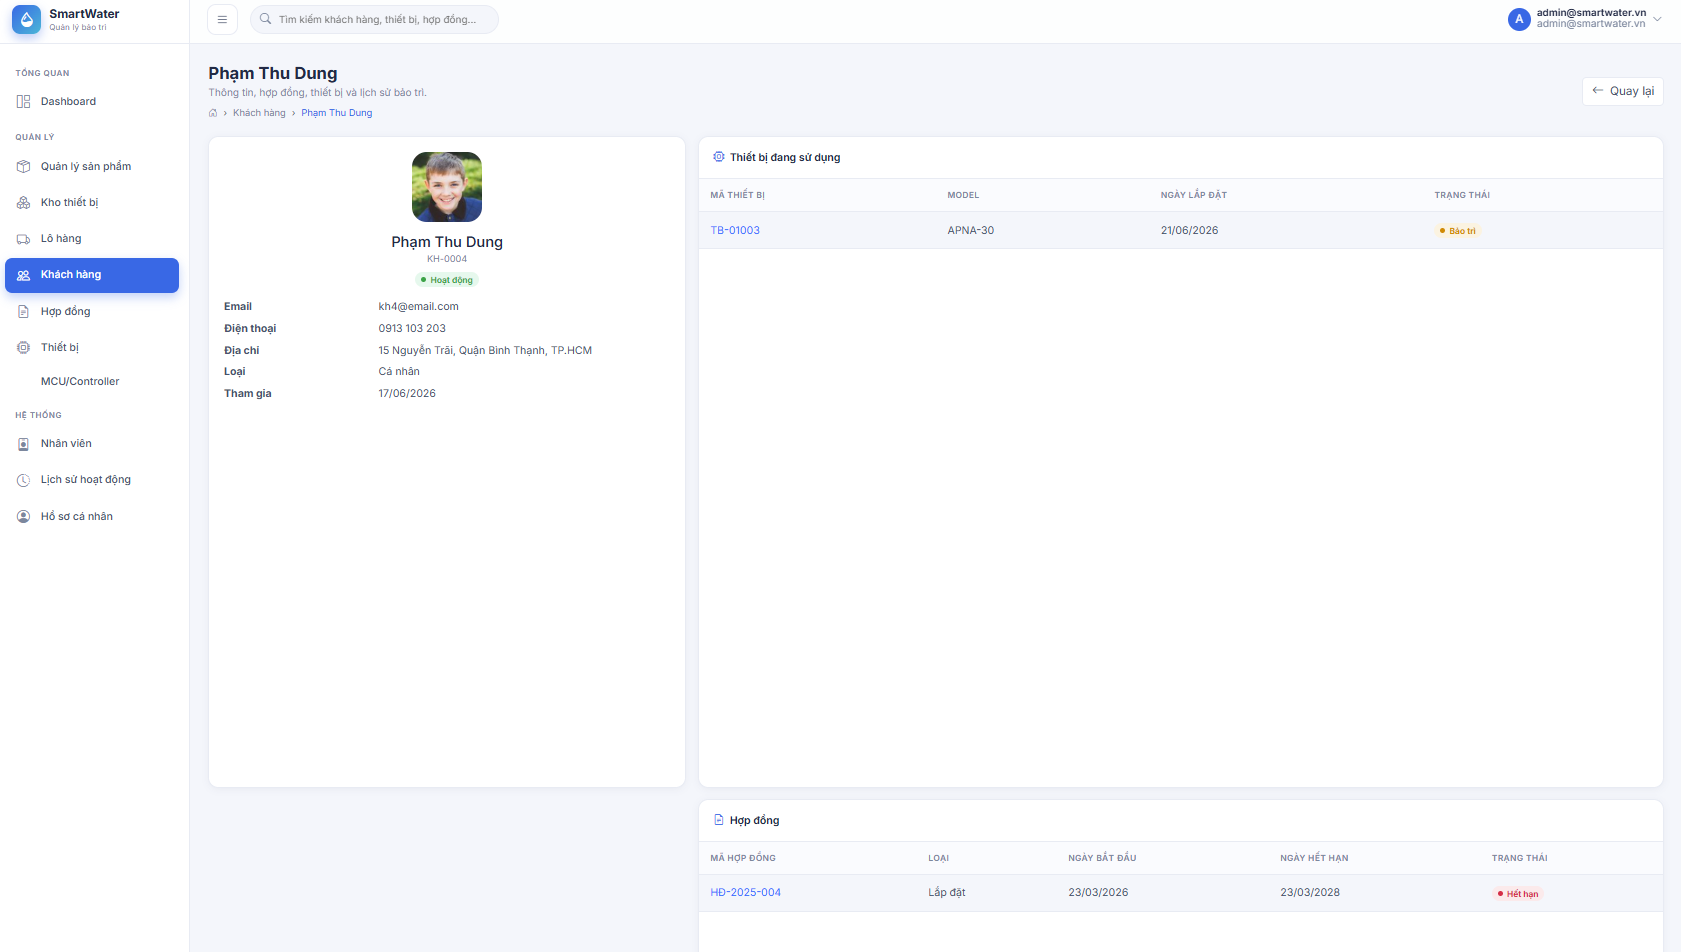
\includegraphics[width=0.90\linewidth]{include/web-UI/smartwater-admin-customer-profile.png}
    \caption{Hồ sơ và thông tin liên quan của khách hàng}
    \label{fig:week7-admin-customer-profile}
\end{figure}

\begin{figure}[H]
    \centering
    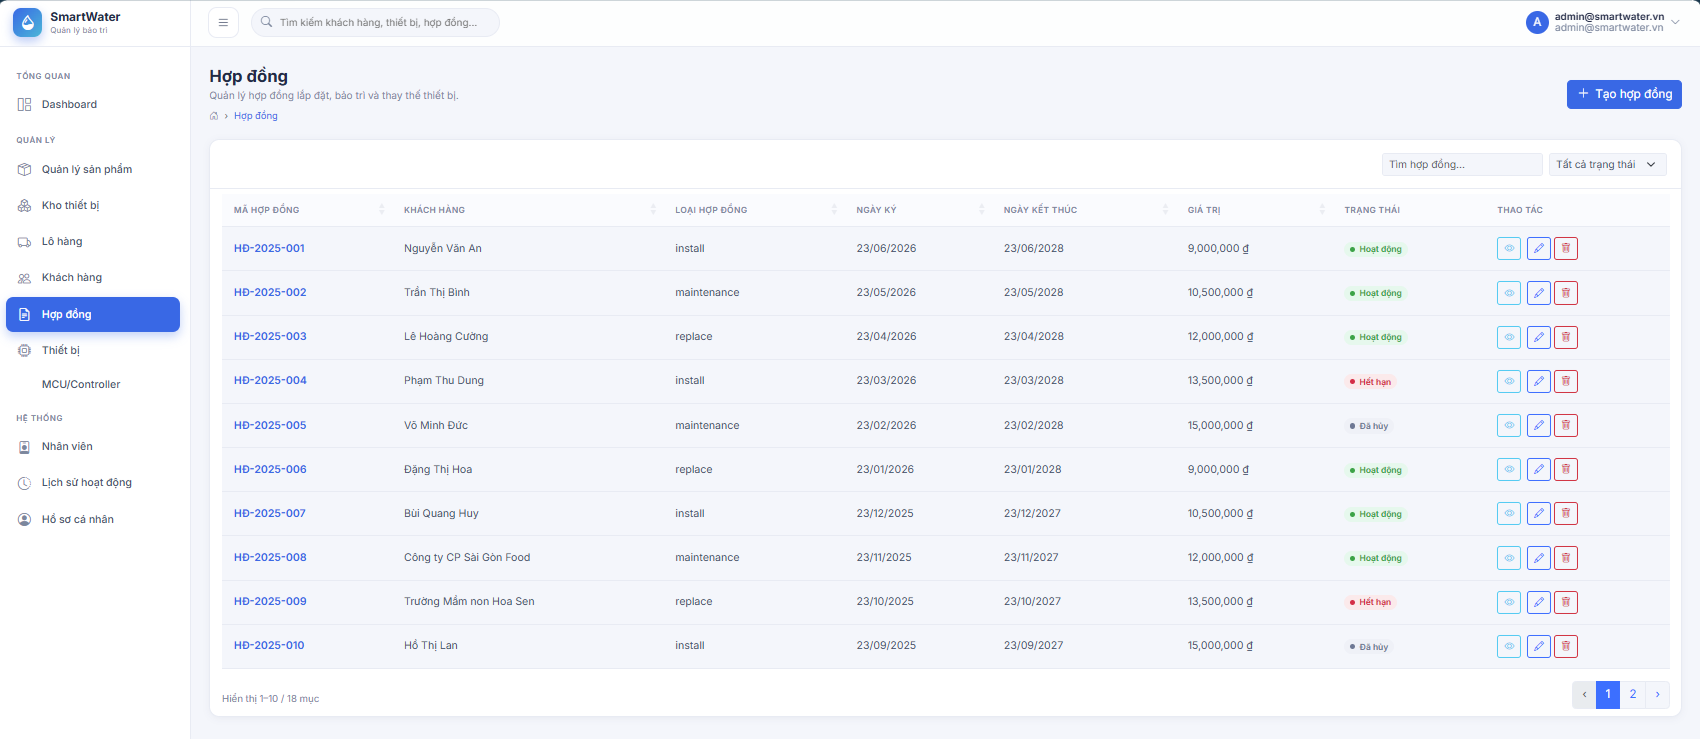
\includegraphics[width=0.90\linewidth]{include/web-UI/smartwater-admin-contract.png}
    \caption{Giao diện quản lý hợp đồng}
    \label{fig:week7-admin-contract}
\end{figure}

\subsubsubsection*{6.2.8.5 Quản lý thiết bị, MCU và telemetry}

Module thiết bị liên kết Product, Customer, Contract và MCU. MCU được nhận diện bằng \texttt{mcu\_id} dạng chuỗi; Device lưu \texttt{mcu\_id} để gắn một MCU vào thiết bị. Khi xem chi tiết thiết bị, dữ liệu telemetry được đọc theo MCU để phục vụ theo dõi TDS và trạng thái cảnh báo.

\begin{figure}[H]
    \centering
    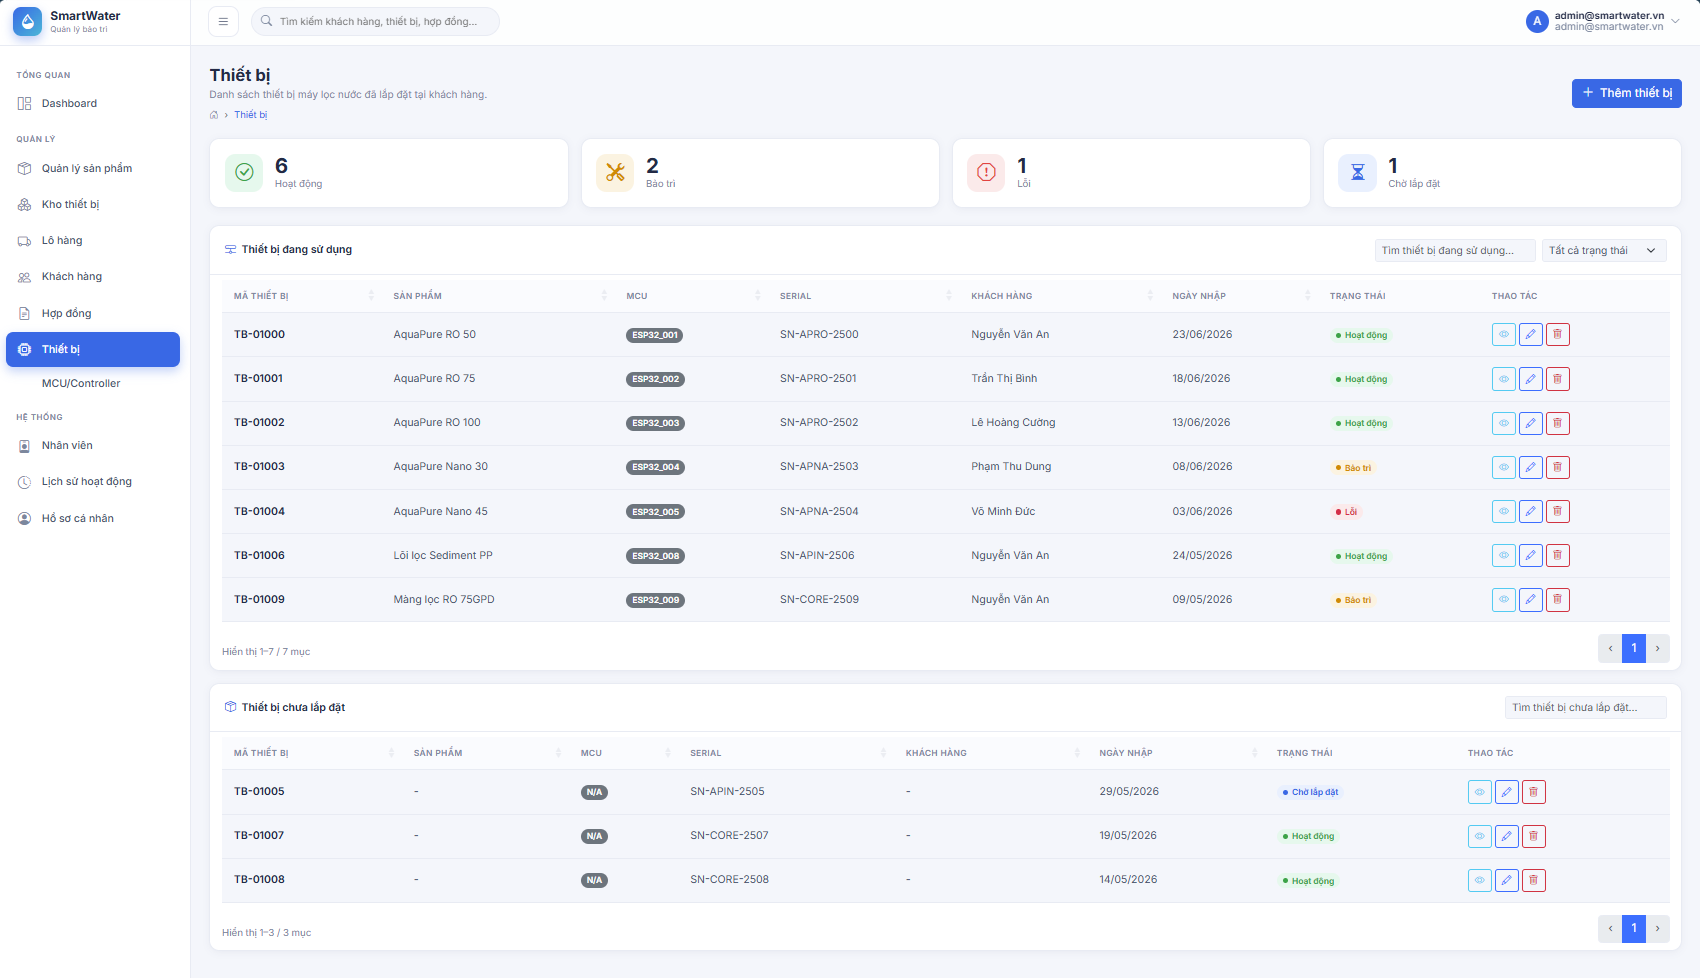
\includegraphics[width=0.90\linewidth]{include/web-UI/smartwater-admin-device.png}
    \caption{Giao diện quản lý thiết bị}
    \label{fig:week7-admin-device}
\end{figure}

\begin{figure}[H]
    \centering
    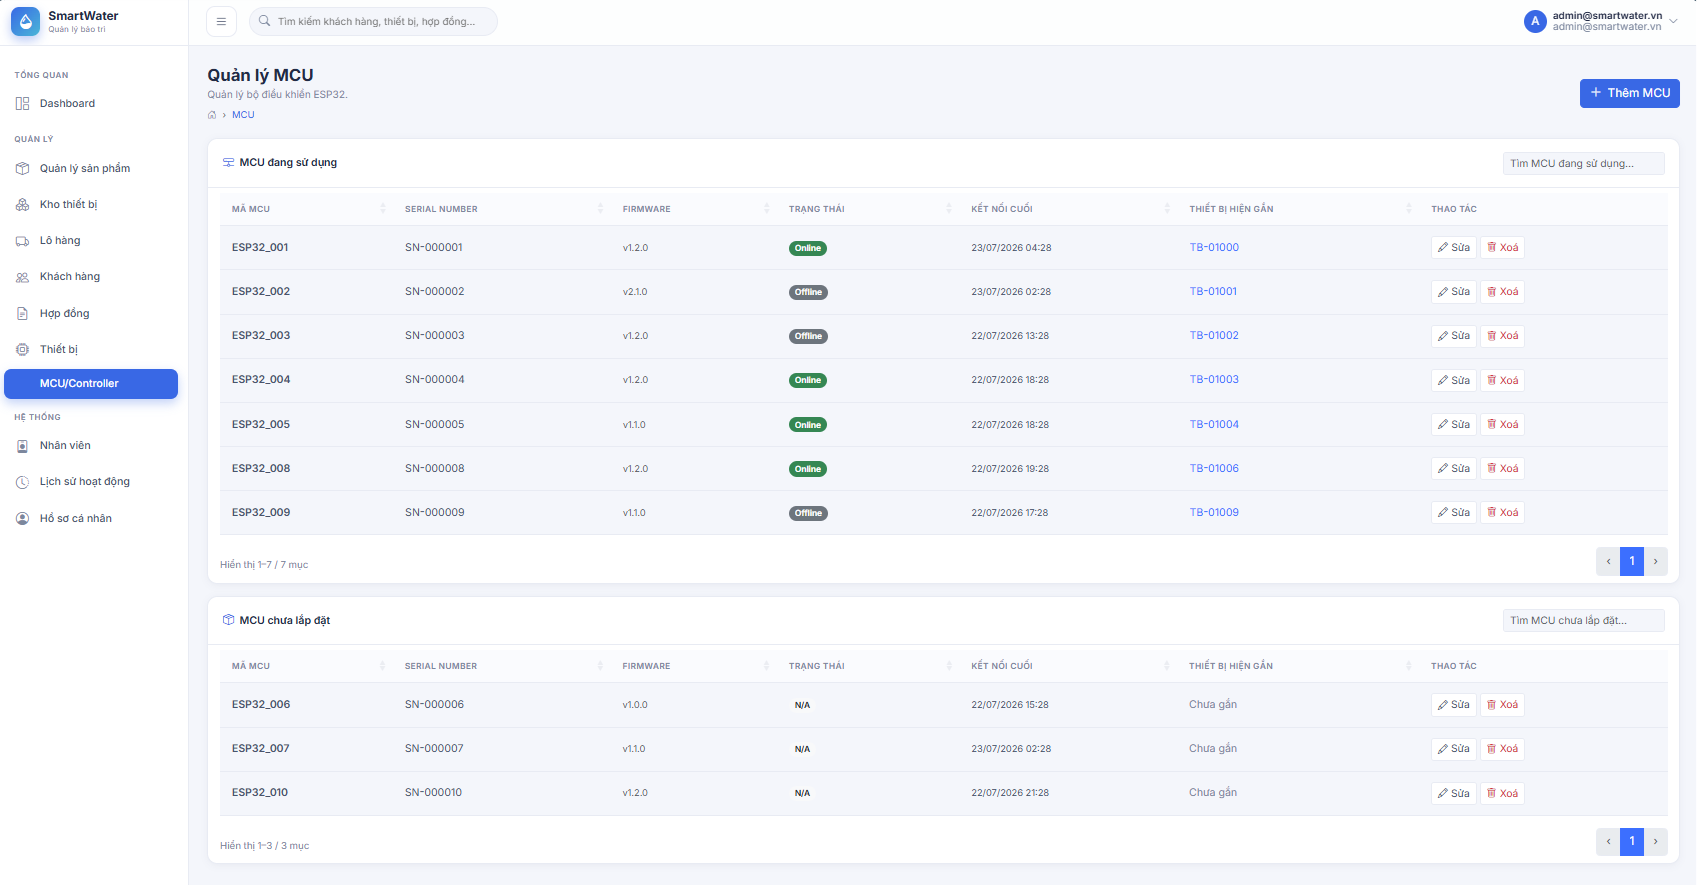
\includegraphics[width=0.90\linewidth]{include/web-UI/smartwater-admin-mcu.png}
    \caption{Giao diện quản lý MCU}
    \label{fig:week7-admin-mcu}
\end{figure}

\begin{figure}[H]
    \centering
    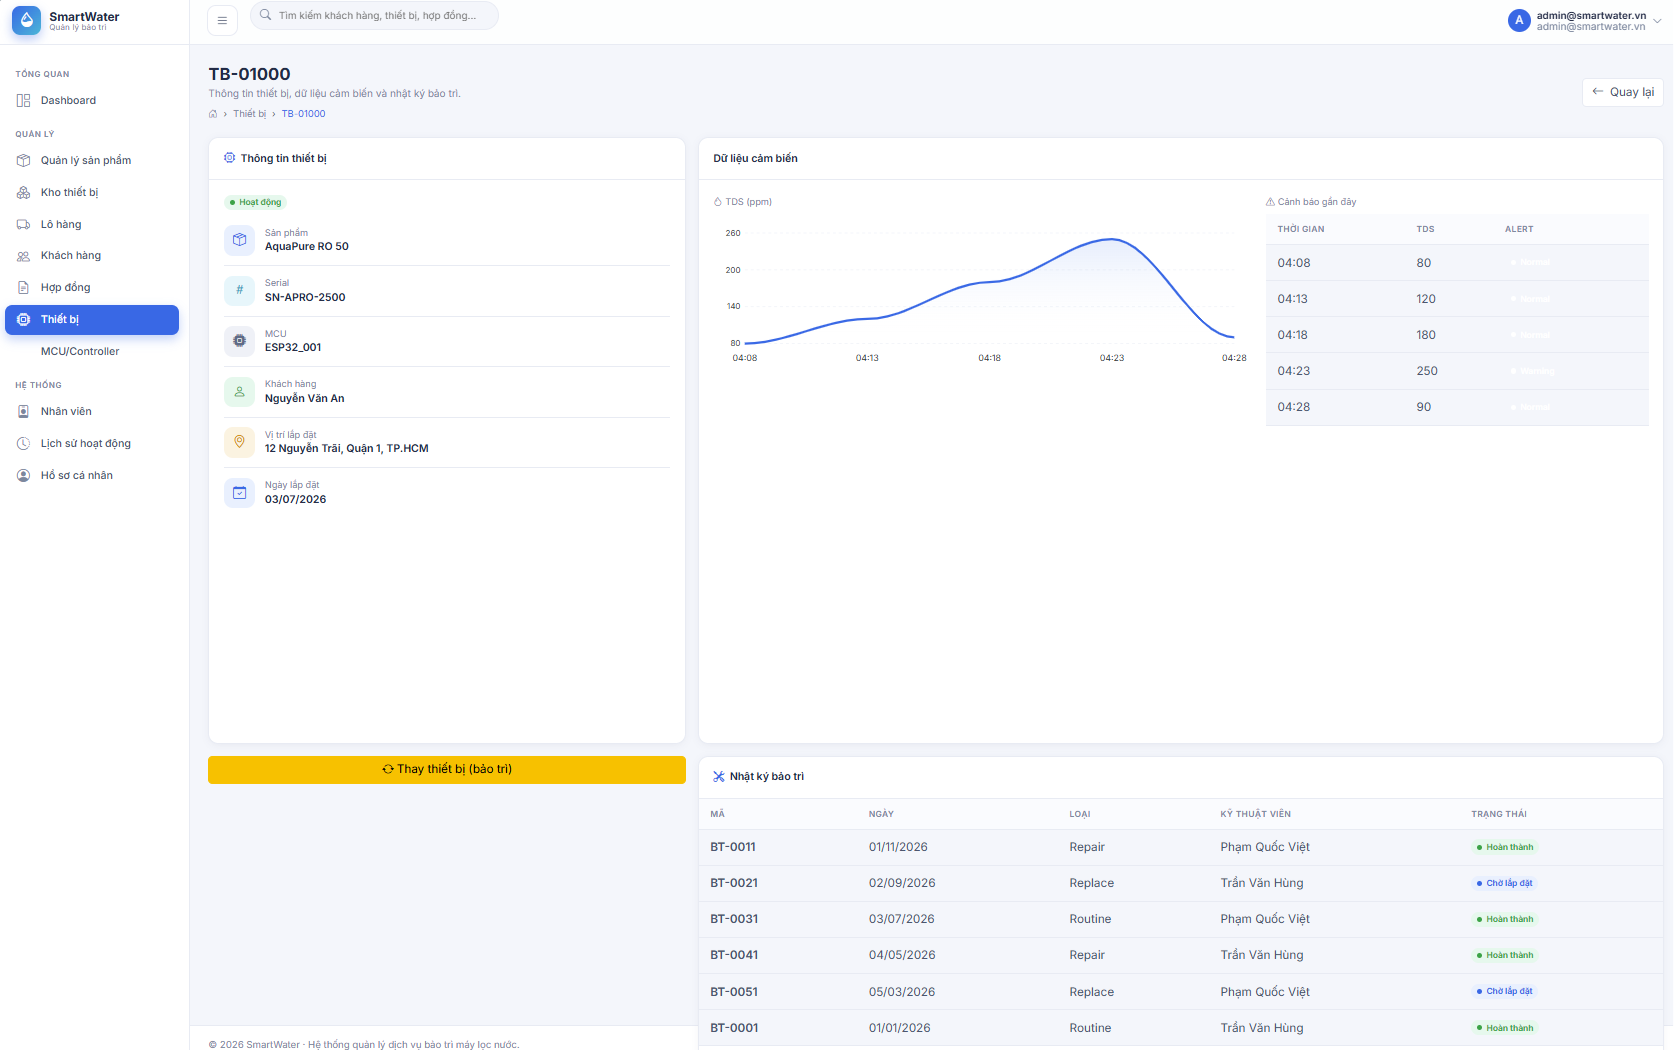
\includegraphics[width=0.90\linewidth]{include/web-UI/smartwater-admin-device-telemetry.png}
    \caption{Telemetry trong màn hình chi tiết thiết bị}
    \label{fig:week7-admin-device-telemetry}
\end{figure}

\subsubsubsection*{6.2.8.6 Nhân viên, hoạt động và hồ sơ người dùng}

Các module nhân viên, lịch sử hoạt động và hồ sơ giúp hỗ trợ vận hành hệ thống. Nhân viên được gắn với vai trò để phân quyền; hoạt động được lưu trong \texttt{activity\_logs}; màn hình hồ sơ cho phép người dùng xem và cập nhật thông tin cá nhân.

\begin{figure}[H]
    \centering
    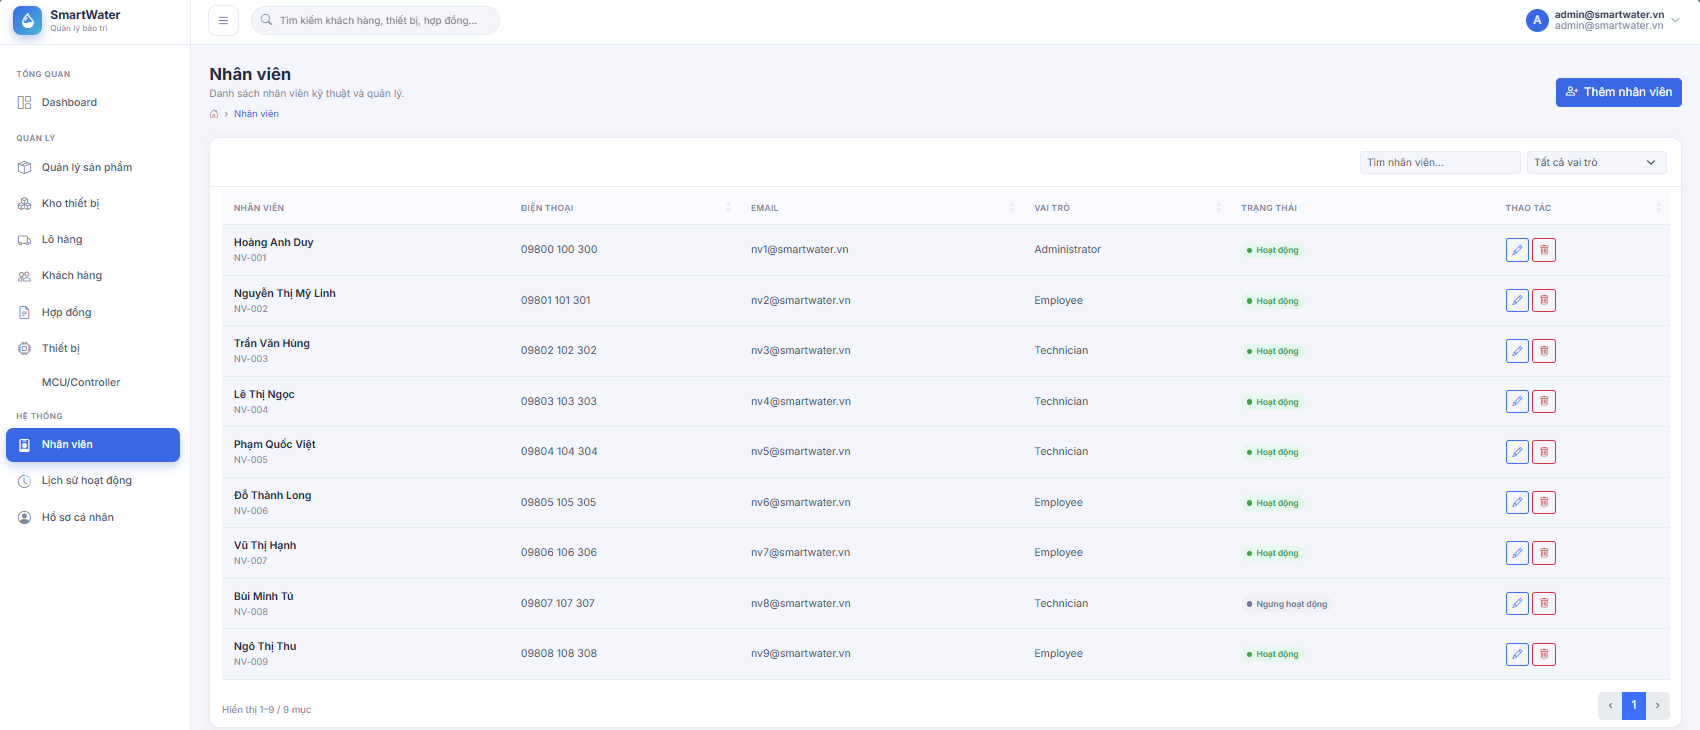
\includegraphics[width=0.90\linewidth]{include/web-UI/smartwater-admin-employee.png}
    \caption{Giao diện quản lý nhân viên}
    \label{fig:week7-admin-employee}
\end{figure}

\begin{figure}[H]
    \centering
    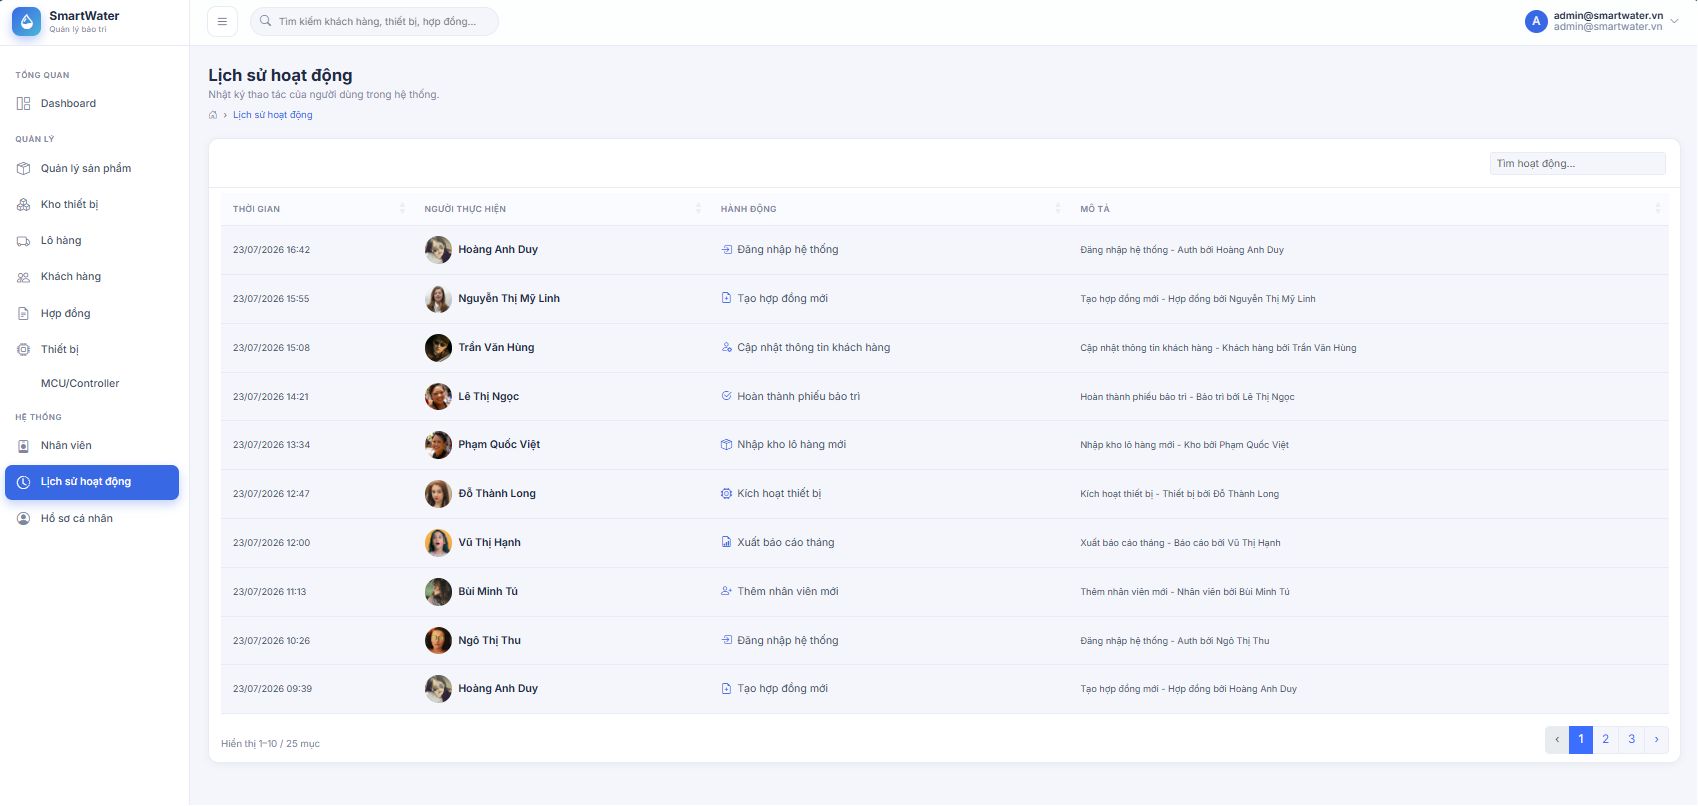
\includegraphics[width=0.90\linewidth]{include/web-UI/smartwater-admin-history.png}
    \caption{Giao diện lịch sử hoạt động}
    \label{fig:week7-admin-history}
\end{figure}

\begin{figure}[H]
    \centering
    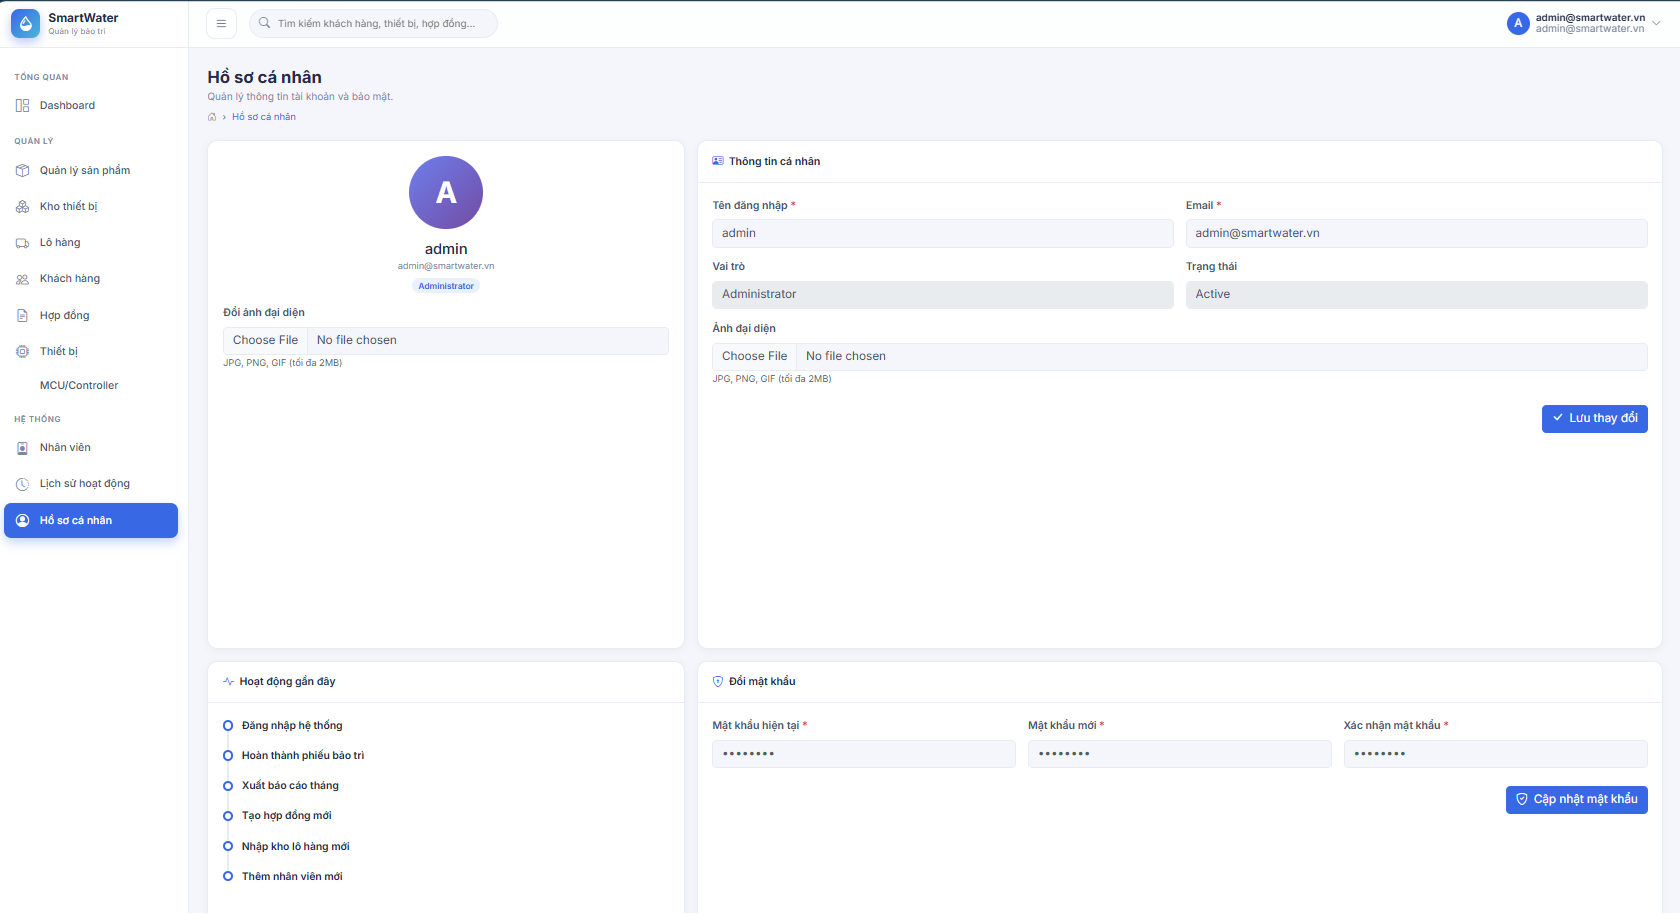
\includegraphics[width=0.90\linewidth]{include/web-UI/smartwater-admin-profile.png}
    \caption{Giao diện hồ sơ người dùng}
    \label{fig:week7-admin-profile}
\end{figure}

\subsubsubsection*{6.3.1 Kết quả xây dựng SmartWater Admin}

Sinh viên kiểm tra luồng điều hướng từ đăng nhập đến các module quản trị, đồng thời đối chiếu dữ liệu hiển thị với các route, controller, service và model của SmartWater Admin. Dashboard có source truy vấn KPI, phân bố thiết bị, khách hàng theo tháng, bảo trì, hoạt động gần đây và hợp đồng sắp hết hạn. Các module sản phẩm, kho, khách hàng, hợp đồng, thiết bị, MCU, nhân viên và hồ sơ đều có màn hình giao diện tương ứng.

Kết quả đạt được:

\begin{itemize}
    \item Hoàn thiện giao diện đăng nhập và dashboard tổng quan cho SmartWater Admin.
    \item Tổ chức các chức năng quản trị theo từng module nghiệp vụ rõ ràng.
    \item Hiển thị được chuỗi dữ liệu Customer--Contract--Product--Device--MCU và telemetry liên quan.
    \item Cung cấp giao diện theo dõi telemetry tại chi tiết thiết bị; dữ liệu TDS được khai thác từ bảng telemetry dùng chung.
    \item Bổ sung các màn hình hỗ trợ vận hành gồm tồn kho, lô hàng, nhân viên, lịch sử và hồ sơ.
\end{itemize}

Phần giao diện quản trị được gộp vào Week 6 để hoàn thiện luồng từ thu nhận telemetry đến khai thác dữ liệu nghiệp vụ. Các phần cần tiếp tục hoàn thiện gồm kiểm thử runtime đầy đủ cho từng module và thay thế xu hướng KPI cố định bằng dữ liệu so sánh thực tế.
